% Das ist die haupt Datei aus der die Ausarbeitung gerneriert wird. Zur besseren übersicht werden die einzellnen Kapitel als eigenen Dateien eingebunden
\documentclass[a4paper,12pt,numbers=noenddot]{scrreprt}
\usepackage[ngerman]{babel}
\usepackage[T1]{fontenc}
\usepackage{lmodern}
\usepackage{cite}
\usepackage{url}
\usepackage{hyperref}
\usepackage{siunitx}
\usepackage{multicol}
\usepackage{xcolor}
\usepackage{graphicx}
\usepackage{pdfpages}
\usepackage[margin=10pt,font=small,labelfont=bf]{caption}
\sisetup{
	locale = DE ,
	per-mode = symbol
}
\usepackage{listings}
\definecolor{codegreen}{rgb}{0,0.6,0}
\definecolor{codegray}{rgb}{0.5,0.5,0.5}
\definecolor{codepurple}{rgb}{0.58,0,0.82}
\definecolor{backcolour}{rgb}{0.95,0.95,0.92}
\definecolor{eclipseStrings}{RGB}{42,0.0,255}
\definecolor{eclipseKeywords}{RGB}{127,0,85}
\colorlet{numb}{magenta!60!black}
\lstdefinestyle{mystyle}{
    backgroundcolor=\color{backcolour},   
    commentstyle=\color{codegreen},
    keywordstyle=\color{magenta},
    numberstyle=\tiny\color{codegray},
    stringstyle=\color{codepurple},
    basicstyle=\ttfamily\footnotesize,
    breakatwhitespace=false,         
    breaklines=true,                 
    captionpos=b,                    
    keepspaces=true,                 
    numbers=left,                    
    numbersep=5pt,                  
    showspaces=false,                
    showstringspaces=false,
    showtabs=false,                  
    tabsize=2
}
\lstdefinelanguage{json}{
    basicstyle=\normalfont\ttfamily,
    commentstyle=\color{eclipseStrings}, % style of comment
    stringstyle=\color{eclipseKeywords}, % style of strings
    numbers=left,
    numberstyle=\scriptsize,
    stepnumber=1,
    numbersep=8pt,
    showstringspaces=false,
    breaklines=true,
    frame=lines,
    %backgroundcolor=\color{gray}, %only if you like
    string=[s]{"}{"},
    comment=[l]{:\ "},
    morecomment=[l]{:"},
    literate=
        *{0}{{{\color{numb}0}}}{1}
         {1}{{{\color{numb}1}}}{1}
         {2}{{{\color{numb}2}}}{1}
         {3}{{{\color{numb}3}}}{1}
         {4}{{{\color{numb}4}}}{1}
         {5}{{{\color{numb}5}}}{1}
         {6}{{{\color{numb}6}}}{1}
         {7}{{{\color{numb}7}}}{1}
         {8}{{{\color{numb}8}}}{1}
         {9}{{{\color{numb}9}}}{1}
}
\lstset{style=mystyle}
\usepackage[printonlyused,withpage]{acronym}
\usepackage[fixlanguage]{babelbib}
\hypersetup{
% TODO: PDF setup
%    bookmarks=true,
    unicode=false,
    pdftoolbar=true,
    pdfmenubar=true,
    pdffitwindow=false,
    pdfstartview={FitH},
    pdftitle={},
    pdfauthor={Nils Robinet},
    pdfsubject={Thema},
    pdfcreator={Nils Robinet},
    pdfproducer={},
    pdfkeywords={} {} {} {},
    pdfnewwindow=true,
    colorlinks=true,
    linkcolor=black,
    citecolor=black,
    filecolor=black,
    urlcolor=black,
%    pagebackref=true
}

\title{Ausarbeitung zum Modul Vertiefung Softwareengineering}
\author{Nils Robinet}

\begin{document}

\maketitle

\tableofcontents

\pagenumbering{arabic}
\setcounter{page}{1}

\chapter*{Abkürzungsverzeichnis}
\begin{acronym}
    \acro{CI/CD}{Continues Integration/Continues Deploy}
    \acro{VM}{Virtual Machine}
    \acro{LTS}{Long Term Service}
\end{acronym}

\chapter{Einleitung}

In dieser Ausarbeitung soll das Abschlussprojekt im Fach \glqq Vertiefung Softwareengineering\grqq{} dokumentiert werden. Im Abschlussprojekt sollte eine \ac{CI/CD} Pipeline aufgesetzt werden und ein Projekt angelegt werden das Beispielhaft über die Pipeline gebaut, gtestet und deployt wird. Als Projekt wurde sich für eine Implementation des Eigengesichtsalogrithmus entschieden. 

Im ersten Kapitel wird beschrieben, wie die Entwicklungsumgebung aufegbaut ist. Im zweiten Kapitel wird kurz auf die git Entwicklungsstrategie eingegangen, mit der das Projekt einwickelt wird. Im Folgenden wird kurz auf die Anwendung, die in dem \ac{CI/CD}-Projekt bebaut wird, eingegangen.
\chapter{Tools}
\label{chap:tools}

Um das Projekt zu bauen werden einige Tools benötigt. Diese sollen hier aufgelistet und ihre Verwendung erklärt werden.
Eine vollständige Liste der Tools die zum bauen des Projekts verwendet werden, kann den Dateien \glqq Dockerfile \grqq{} und \glqq requirements.txt \grqq{} entnommen werden.

\begin{description}
    \item[pdflatex] ist ein Typesetter der verwendet wird um aus laTeX markup PDF Dokumente zu erzeugen. Es wird hier verwerndet, um dieses PDF Dokument zu erstellen. \cite{MANLATEX}.
    \item[Marp] ist eine Umgebung, um aus Markdown Präsentationen zu generieren. Es wird verwendet, um für die Päsentation zur Ausarbeitung ein PDF zu erstellen \cite{MARP2024}.
    \item[Jenkins] ist ein System zur Umsetzung von \glqq contiues integratio \grqq{} und \glqq continues deployment\grqq{} von Software \cite{JENKINS2024}.
    \item[gcc / g++] Die GNU Compiler Collection ist eine Sammlung von Kompilern, insbesondere für die Programmiersprachen der C Familie\cite{GCC2024}. Sie wird in diesem Projekt zum übersetzen von C++ Code genutzt.
    \item[CMake / Make] CMake ist ein Meta Build Generator, der genutzt wird um die eigentlichen Build Generatoren wie Make zu konfigurieren. Make wird genutzt um das eigentliche Bauen und Linken von Programmen zu vereinfachen\cite{CMAKE2024}.
    \item[cython] Cython ist ein Werkzeug, das es ermöglicht C/C++ Erweiterungen für Python einfach zu programmieren. Cython kompiliert Python und die Cython-Programmiersprache in C/C++ Code, der mit allen gängigen C/C++-Kompilern kompiliert werden kann. Herauskommen CPython kompatible Shared-Library-Objekte\cite{behnel2011}.
    \item[Docker] Docker ist eine Container-Engine, die es ermöglicht Anwendungen zu Isolieren und ihnen eine stabile Laufzeitumgebung zu garantieren. In einen Container kann eine Anwendung mit all ihren Abhängigkeiten gepackt werden. So ist ein Einfacher Transport und Auslieferung möglich\cite{merkel2014}.
\end{description}

\chapter{Entwicklungsumgebung}

Für das Projekt sollte eine \acf{CI/CD} Pipline angelegt werden. Zu diesem Zweck wird ein Build Server in einer \acf{VM} gestartet.

\section{Werkzeuge und Anwendungen}

Der Code des projektes wird mit der Versionsverwaltungssoftware GIT gemanaged (mehr zur git Strategie in chap TODO). Um das remote repository zu managen wird auf Github gesetzt. Die \ac{CI/CD} Pipeline wird durch den open source Build-Server Jenkins gemanaged. Die Build-Toolchain wird in einem Docker-Container bereit gestellt. Der Build-Server läuft in einer \ac{VM}. Als Virtualisierungslösung wurde QEMU/KVM ausgeählt. Die Builds werden mittels CMake und Bash-Scipten Konfiguriert.

\section{Build-Server Setup}

Als Guest-Beriebsystem wurde sich für Arch Linux entschieden, da von diesem Betriebsystem bereits fertig vorgebaute \ac{VM} images bereit gestellt werden (\url{https://gitlab.archlinux.org/archlinux/arch-boxes/-/packages}). Unter anderem wird ein qcow2 image das in der Virtualisierungsumgebung QEMU eingesetzt werden kann bereit gestellt.
In der \ac{VM} wird ein Jenkins build server installiert, der die CI/CD pipline bedient.

\subsection{Installation}

Die Build-Server \ac{VM} wurde auf ein Arch Linux System erstellt, einzellne Schritte, insbesondere wenn eine Packetverwaltungssoftware eingesetzt wird können sich zwischen den verschiedenen Betriebsystemen unterscheiden.
Zur erstellung und installation wurden folgende Schritte durch geführt:

\begin{enumerate}
    \item Datenträgerabbild herunter laden:\\
        \lstinline[language=sh]!wget -O build_server.qcow2 https://gitlab.archlinux.org/archlinux/arch-boxes/-/package_files/6852/download!
    \item Virtuelle Machine Starten:\\
    \lstinline[language=sh]!qemu-system-x86_64 -m 4G -smp 4 -enable-kvm\! \\
    \lstinline[language=sh]!                   -nic user,hostfwd=tcp::60022-:22,hostfwd=tcp::8090-:8090\ !\\
    \lstinline[language=sh]!                   build_server.qcow2!\\
    Der Benutzername und das Standartpasswort lauten: arch/arch; Man kann sich nun mittels ssh mit der \ac{VM} verbinden:\\
    \lstinline[language=sh]!ssh arch@localhost -p 60022!\\
    \item Jenkins installieren:\\
    \lstinline[language=sh]!pacman -Syu !\\
    \lstinline[language=sh]!pacman -S fontconfig!\\
    \lstinline[language=sh]!pacman -S freetype2!\\
    \lstinline[language=sh]!pacman -S jenkins!\\
    \lstinline[language=sh]!pacman -S docker!\\
    \lstinline[language=sh]!pacman -S git!\\
    \lstinline[language=sh]!systemctl enable jenkins!\\
    \lstinline[language=sh]!systemctl enable docker!\\
    \lstinline[language=sh]!systemctl start jenkins!\\
    \lstinline[language=sh]!systemctl start docker!\\
    \lstinline[language=sh]!sudo usermod -aG docker jenkins!\\
    \item Nach der installation kann über den Webrowser auf dem Host Beriebsystem unter der Addresse http://localhost:8090 auf die jenkins installation zu gegriffen werden. Im initialen Setup-dialog muss ausgewählt werden ob dieStandar-Plugins installiert werden sollen, hier sollte mit ja geantwortet werden, und ein Admin Benutzer angelegt werden. Danach landet man im Haupmenu der Jenkins installation.

Zusätzlich wird noch das Plugin "Docker Pipeline" benötigt, das es ermöglicht in docker images zu bauen.
\end{enumerate}

\subsection{Projekt einrichtung}

Unter dem Punkt "new job" wird ein neuer Multibranch Pipeline Job angelegt und Konfiguriert. Als Branch Source wird das github Repo dieses Projekts angegeben. Damit jenkins auf das Projekt zu greifen kann müsen noch Github credentials eingrtragen werden. 

Damit Jenkins Änderungen zeitnah erkennt wir ein periodischer Trigger mit einem Intervall von einer Minute eingestellt. Danach ist das Projekt fertig konfiguriert und kann benutzt werden.

Die Build und Deployment stages werden durch das im Repositroy eingecheckte Jenkinsfile konfgiuriert. Der build findet in einem Docker-Container statt der durch ein Dockerfile, das ebenfalls eingecheckt ist, erstellt wird. Das docker image wird durch Jenkins gemanaged, Jenkins kümmert sich auch darum das Dockerimage beiÄnderungen am Dockerfile neu zu generieren.

\chapter{Entwicklungsstartegie}
\label{chap:git-strat}

Das Projekt wird auf mehreren Branches entwickelt um eine saubere Trennung zwischen Entwickung und produktivem Code zu gewährleisten. Dazu wird auf die GitFlow branching Strategie gesetzt. Hierbei gibt es zwei Hauptbranches: 

Zum einen den main branch der den produktiven Code enthält und dessen build Artifakte in die prokutive Umgebung deployed werden und den develop Branch auf dem die aktive Entwicklung stattfindet. Einzellne features werden auf so gennanten Feature-Branches entwickelt. Ist ein Feature fertig entwickelt, kann es auf dem develop branch integriert werden. Auf dem develop branch können dann auch umfassendere Tests laufen die sicher stellen, dass das zurück merges des Feature-Branches nicht zu einer Destabilisierung des gesammt Systems geführt hat. Wenn der develop Branch alle Tests duchlaufen hat und alle Features die für den nächsten Release gewünscht waren fertig entwickelt sind, wird der develop in den main Branch zurück gemerged, was zu einem neuen Release führt.

Zusätzlich gibt es für schnelle Paches von wichtigen Fehlern die Möglichkeit hotfix Branches anzulegen, die direkt in den main Branch gemerged werden dürfen.

Wenn mehrere Entwickler an einem Projektm das eine solche Branching-Strategie verfolgt, arbeiten, dann sollten Branch-Protection-Rules eingesetzt werden um die beiden Hauptbranches zu schützen. So bietet es sich z.B. an dann für einen Merge auf develop oder main immer ein Reviewer einen den Pull-Request genehmigen muss. Außderdem kann es sinnvoll sein, dass bestimmte Tests nicht ausfallen dürfen bevor auf den develop oder main branch gemerged wird.

\begin{figure}
    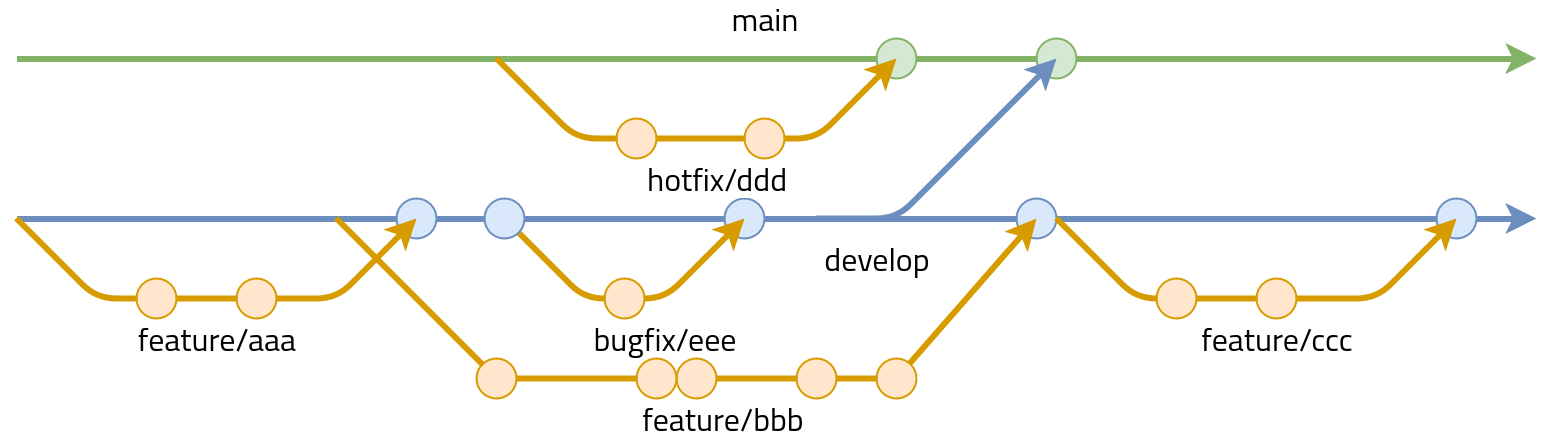
\includegraphics[scale=0.25]{res/branching_scheme.drawio.png}
    \caption{Vereinfachte Darstellung eines Branch-Graphs bei Anwendung des beschriebenen Branching Schemas.}
\end{figure}
\chapter{Anwendung}

Um die verwendung der \ac{CI/CD}-Pipeline zu demonstrieren soll ein Projekt angelegt werden, welches über rudimentäre Funtionen verfügt.
Es wurde sich dazu Entschieden eine python-kompatible Bibliothek zur Verdwendung des Eigenface Alogrithmus zu entwicken. Um deren Effektivität demonstrieren zu können soll eine Demoanwendung in Form einer Webseite, die im Backend die Bibliothek verwendet und dem Nutzer die möglichkeit gibt die Funktionaliteten der Bibliothek aus zu probieren, bereit gestellt werden. Die Demo Webanwendung soll durch die \ac{CI/CD}-Pipeline in einem Docker-Container installiert und deployed werden.

\section{Eigenface-Bibliothek}

Der Eigenface Algorithmus soll aus Performance gründen in C++ implementiert werden (Für die Dokumnetation der C++ implementierung siehe \autoref{chap:doxy}). Um das Interfacing mit Python zu vereinfachen soll mit Hilfe der Programmiersprace Cython (Siehe \autoref{chap:tools}) eine Schnittstelle implementiert werden, die aus aus Python aufrufbaren Klassen und Funktionen bereit stellt.

Die C++ Implementation soll über Unit tests, die von der CI/CD Pipeline automatisiert aufgerufen werden, abgesichert werden. Hierzu soll zu jeder Funkion ein Test vorliegen. Die Unit tests sollen im Google Test Framework unmgestzt werden. Für die Auswertung soll ein junit kompatibles XML generiert werden.

Das Cython interface soll mit Hilfe des pytest Frameworks getestet werden. Hier sollen nur high-level tests implementiert werden, die nicht unbedingt die Funktionalität der C++ Funktionen testen, sondern ihren Fokus auf die Absicherung der Schnittstellen legen. Auch die Python Tests sollen ein junit kompatibles XML generieren.

\section {Demo Anwendung}

Die Demo Anwendung soll eine Webseite sein auf der ein interessierter Nutzer die Grundfunktionalitäten der Eigenface Bibliotheke ausprobieren kann. Um die webseite bereit zustellen und die Python-Schnittstellen der Bibliothek zu nutzen soll eine Webserver Anwendung mithilfe des freien Cherrypy Frameworks \ref{TODO} erstellt werden.
Die demoanwdung soll mit pylint überprüft werden, um sicher zu stellen, dass der Code gängigen Codestyle Guildlines entspricht. Abweichend vom Standart soll camel-case (camelCase) anstelle con snake-case (snake\_case) verwendet werden. Hierzu wird eine pylintrc Datei im Repository bereit gestellt. Zur besseren Visualisierung der Testergebnisse soll das Modul pylint-junit eingesetzt werden, dass die Ergbnisse des Lint-Vorgangs im Junit-XML format ausgibt.

\appendix
    \includepdf[pages=-]{../../build/docu/latex/refman.pdf}
\end{document}
